\documentclass[border=10pt]{standalone}

\usepackage{tikz}
\usepackage{tikzsymbols}
\usetikzlibrary{calc,patterns,shapes.geometric}

\def\centerarc[#1](#2)(#3:#4:#5){\draw[#1] ($(#2)+({#5*cos(#3)},{#5*sin(#3)})$) arc (#3:#4:#5);}

\begin{document}
	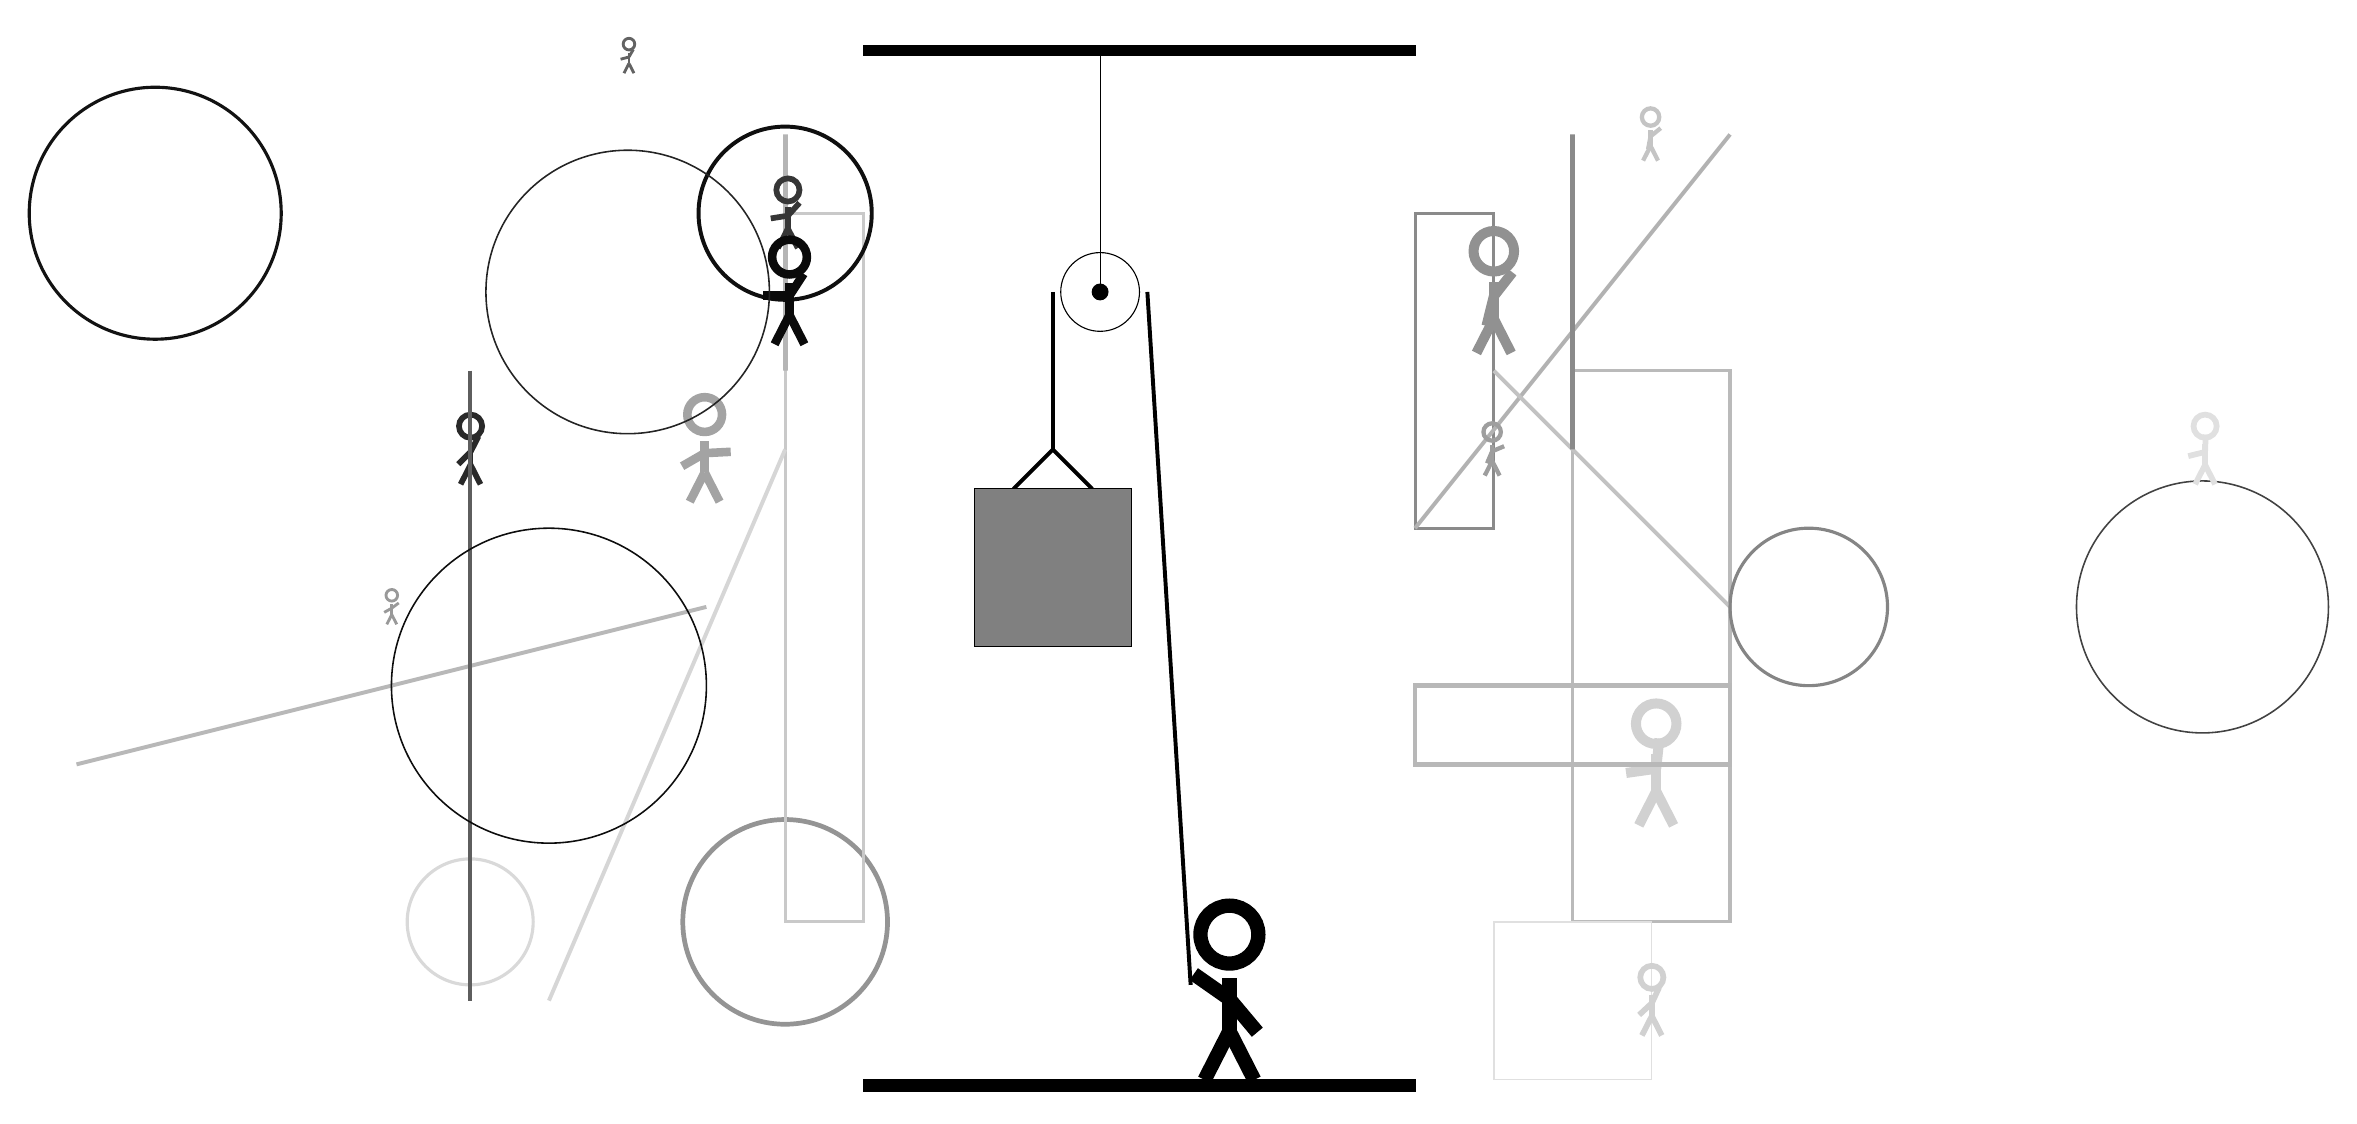
\begin{tikzpicture}
		%%%%% START %%%%%
		
		\draw[fill=black] (-2, 10) rectangle (5, 10.125);
		
		\draw[line width=0.4mm, color=black!46] (6, 8) rectangle (5, 4);
		
		\draw[line width=0.4mm, color=black!27] (7, 6) rectangle (9, -1);
		\node[line width=0.2mm, color=black!40] at (-8, 3) {\Strichmaxerl[2][29][37]};
		\draw[line width=0.5mm, color=black!30](5, 4) -- (9, 9);
		
		\draw [line width=0.6mm, color=black!42](-3, -1) circle (1.3);
		\draw[line width=0.4mm, color=black!21] (-3, 8) rectangle (-2, -1);
		
		\draw[line width=0.5mm, color=black!16](-6, -2) -- (-3, 5);
		\draw [line width=0.4mm, color=black!15](-7, -1) circle (0.8);
		\draw[line width=0.5mm, color=black!24](6, 6) -- (9, 3);
		
		\node[line width=0.3mm, color=black!36] at (-4, 5) {\Strichmaxerl[6][30][3]};
		\draw[line width=0.5mm, color=black!28](-4, 3) -- (-12, 1);
		\draw[line width=0.6mm, color=black!29] (-3, 6) rectangle (-3, 9);
		\node[line width=0.6mm, color=black!79] at (-3, 8) {\Strichmaxerl[4][9][48]};
		
		\draw [line width=0.4mm, color=black!48](10, 3) circle (1.0);
		\draw [line width=0.5mm, color=black!94](-3, 8) circle (1.1);
		\node[line width=0.6mm, color=black!43] at (6, 7) {\Strichmaxerl[7][76][52]};
		\node[line width=0.4mm, color=black!96] at (-3, 7) {\Strichmaxerl[6][0][57]};
		\draw [line width=0.4mm, color=black!93](-11, 8) circle (1.6);
		\node[line width=0.6mm, color=black!18] at (8, 1) {\Strichmaxerl[7][8][84]};
		
		\node[line width=0.4mm, color=black!84] at (-7, 5) {\Strichmaxerl[4][45][63]};
		\draw[line width=0.2mm, color=black!12] (6, -3) rectangle (8, -1);
		
		\node[line width=0.4mm, color=black!61] at (-5, 10) {\Strichmaxerl[2][15][60]};
		\draw [line width=0.2mm, color=black!86](-5, 7) circle (1.8);
		\draw[line width=0.5mm, color=black!63](-7, 6) -- (-7, -2);
		\draw[line width=0.6mm, color=black!28] (5, 1) rectangle (9, 2);
		
		\draw [line width=0.2mm, color=black!95](-6, 2) circle (2.0);
		
		\node[line width=0.7mm, color=black!38] at (6, 5) {\Strichmaxerl[3][67][23]};
		\node[line width=0.2mm, color=black!18] at (8, -2) {\Strichmaxerl[4][43][65]};
		\draw [line width=0.2mm, color=black!74](15, 3) circle (1.6);
		\node[line width=0.5mm, color=black!23] at (8, 9) {\Strichmaxerl[3][79][39]};
		\node[line width=0.5mm, color=black!12] at (15, 5) {\Strichmaxerl[4][14][88]};
		\draw[line width=0.6mm, color=black!46] (7, 5) rectangle (7, 9);
		
		\draw (1, 7) circle (0.5);
		\draw[fill=black] (1, 7) circle (0.1);
		\draw (1, 10) -- (1, 7);
		
		\draw[line width=0.5mm] (-0.1, 4.5) -- (0.4, 5.0) -- (0.9, 4.5);
		\draw[fill=black!50] (-0.6, 4.5) rectangle (1.4, 2.5);
		
		\draw[line width=0.5mm] (0.4, 7) -- (0.4, 5.0);
		\centerarc[line width=0.5mm](1, 7)(0:180:0.6);
		\draw[line width=0.5mm](1.6, 7) -- (2.15, -1.8);
		
		\node at (2.6, -1.9) {\Strichmaxerl[10][-35][-50]};
		
		\draw[fill=black] (-2, -3) rectangle (5, -3.15);
		
		%%%%% END %%%%%
	\end{tikzpicture}
\end{document}